\documentclass[12pt]{article}
\usepackage[margin=1in]{geometry}
\usepackage{amsmath,amssymb,mathtools}
\usepackage{enumitem}
\usepackage{bm}
\usepackage{hyperref}
\usepackage{fancyhdr}
\usepackage{draftwatermark}
\usepackage{xcolor}
\usepackage{pgfplots}
\usepackage{titlesec}
\pgfplotsset{compat=newest}

%------------- TITLE AND METADATA -------------
\newcommand{\CourseCode}{HE2001 }
\newcommand{\CourseName}{Microeconomics II}
\newcommand{\DocType}{Tutorial 7}

\title{
\CourseCode \CourseName \\[0.3em]
\large \DocType
}
\author{
  Academic Year 2025/2026, Semester 2 \\[0.25em]
  \textit{Quantitative Research Society @NTU}
}
\date{\today}

%------------- HEADER & FOOTER (for page 2 onward) -------------
\fancypagestyle{main}{
  \fancyhf{}
  \fancyhead[L]{\CourseCode \CourseName \ --\ \DocType}
  \fancyhead[R]{\href{https://qrsntu.org}{QRS@NTU}}
  \fancyfoot[C]{\thepage}
  \renewcommand{\headrulewidth}{0.4pt}
  \renewcommand{\footrulewidth}{0pt}
}

%------------- SIMPLE FOOTER (page 1 only) -------------
\fancypagestyle{plainfirst}{
  \fancyhf{}
  \renewcommand{\headrulewidth}{0pt}
  \renewcommand{\footrulewidth}{0pt}
  \fancyfoot[C]{\scriptsize\textcolor{gray}{\textit{For academic reference only. This document is provided for educational purposes and does not constitute an official question paper, answer key, or any formally authorised academic material. Its content is not guaranteed to be complete or accurate.}}}
}

%------------- WATERMARK -------------
\SetWatermarkText{Unofficial — QRS@NTU — qrsntu.org}
\SetWatermarkScale{1}
\SetWatermarkLightness{0.99}

%------------- SHORTCUTS -------------
\newcommand{\R}{\mathbb{R}}
\newcommand{\Rp}{\mathbb{R}_+}
\newcommand{\E}{\mathbb{E}}
\newcommand{\Var}{\mathrm{Var}}
\newcommand{\dotp}{\cdot}

%------------- STYLE -------------
\setlist[enumerate]{itemsep=0.32em, topsep=0.32em}
\setlist[itemize]{itemsep=0.22em, topsep=0.22em}

\titleformat{\subsubsection}[block]
{\normalfont\large\bfseries}
{}
{0pt}
{}

\titleformat{\paragraph}[block]
{\normalfont\normalsize\bfseries}
{}
{0pt}
{}

\titlespacing*{\paragraph}
{0pt}
{1.2ex}
{0.6ex}

\setcounter{secnumdepth}{0}
\setcounter{tocdepth}{4}

\begin{document}

\maketitle
\thispagestyle{plainfirst}
\pagestyle{main}
\bigskip

%====================================================
% OVERVIEW
%====================================================
\begin{center}
  \rule{0.8\textwidth}{0.4pt}\\[4pt]
  \textbf{Overview}\\[2pt]
  \rule{0.8\textwidth}{0.4pt}
\end{center}

\noindent
This tutorial covers:
\begin{itemize}[leftmargin=*]
  \item welfare analysis for price changes under perfect complements, quasilinear utility, and Cobb--Douglas utility;
  \item Hicksian and Marshallian demand, together with equivalent variation (EV) and compensating variation (CV);
  \item reservation prices and inverse demand under quasilinear preferences;
  \item indirect utility and expenditure-based welfare calculations;
  \item consumer surplus and its relation to EV and CV;
  \item past-year style applications involving price changes and discrete-choice quasilinear utility.
\end{itemize}

\bigskip

\newpage
\tableofcontents


%====================================================
% QUESTION 1
%====================================================
\section{Question 1: Bernice and Welfare Measures}

\noindent
Bernice’s preferences can be represented by \(u(x, y)=\min\{x, y\}\), where \(x\) is pairs of earrings and \(y\) is dollars to spend on other things. She faces prices \((p_x, p_y)=(2,1)\) and her income is \(12\).

\subsection{Problem}
\begin{enumerate}[label=(\alph*)]
    \item Draw in a graph, her budget constraint and several indifference curves, illustrating the optimal bundle.
    \item The price of a pair of earrings rises to \$3 and Bernice’s income stays the same. On the same graph, draw her new budget constraint, illustrating the optimal point.
    \item What bundle would Bernice choose if she faced the original prices and had just enough income to reach the new indifference curve in (b)? Draw a budget line which passes through this bundle at the original prices. What is the level of income Bernice has at this new budget line?
    \item What is the equivalent variation (EV) of the price increase in earrings from \$2 to \$3? Remember that EV is the maximum income that at the original prices, when removed, just gives the consumer the same final utility level.
    \item What bundle would Bernice choose if she faced the new prices and had just enough income to reach the original indifference curve in (a)? Draw a budget line which passes through this bundle at the new prices. What is the level of income Bernice has at this budget line?
    \item What is the compensating variation (CV) of the price increase in earrings from \$2 to \$3 ? Remember that CV is the least income that at the new prices, when given, just restores the consumer’s original utility level.
\end{enumerate}

\newpage
\subsection{Solution}

\subsubsection{Method 1: ATQ-focused utility maximisation}
\begin{enumerate}[label=(\alph*)]
    \item
    Since
    \[
    u(x,y)=\min\{x,y\},
    \]
    Bernice has Leontief preferences, so at the optimum she chooses the kink:
    \[
    x=y.
    \]
    Her budget constraint is
    \[
    2x+y=12.
    \]
    Substituting \(y=x\),
    \[
    2x+x=12
    \;\Longrightarrow\;
    3x=12
    \;\Longrightarrow\;
    x=4.
    \]
    Hence
    \[
    y=4.
    \]
    Therefore the optimal bundle is
    \[
    \boxed{(4,4)}
    \]
    and the original utility level is
    \[
    \boxed{u_0=4.}
    \]

    A correct graph should show:
    \begin{itemize}[leftmargin=*]
        \item the original budget line \(2x+y=12\);
        \item several L-shaped indifference curves;
        \item the optimal point \((4,4)\).
    \end{itemize}

    \begin{center}
    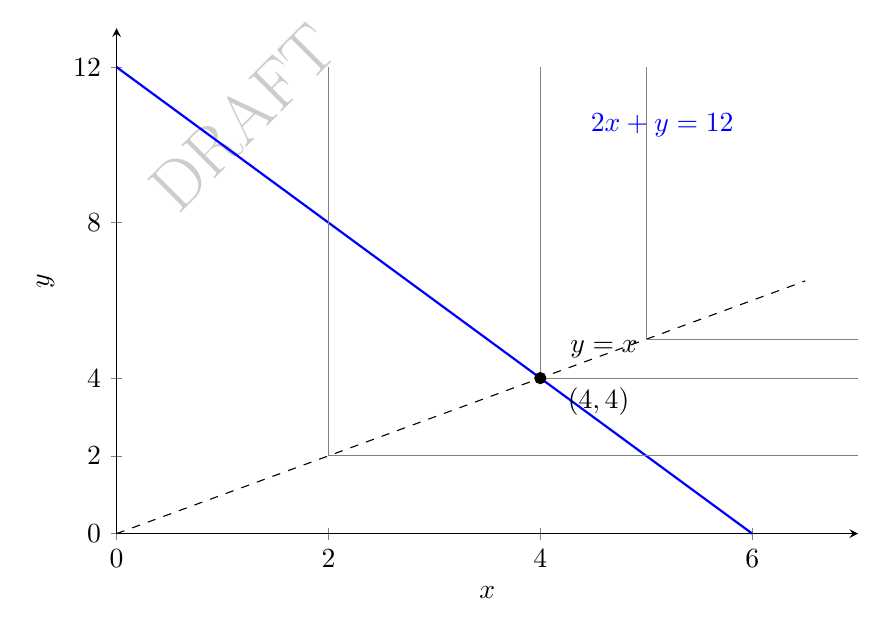
\begin{tikzpicture}
    \begin{axis}[
        width=11cm,
        height=8cm,
        xmin=0,xmax=7,
        ymin=0,ymax=13,
        axis lines=left,
        xlabel={$x$},
        ylabel={$y$},
        xtick={0,2,4,6},
        ytick={0,2,4,8,12},
        clip=false
    ]
    \addplot[domain=0:6,samples=2,thick,blue] {12-2*x};
    \addplot[dashed,domain=0:6.5,samples=2,black] {x};

    \addplot[gray] coordinates {(2,12) (2,2) (7,2)};
    \addplot[gray] coordinates {(4,12) (4,4) (7,4)};
    \addplot[gray] coordinates {(5,12) (5,5) (7,5)};

    \addplot[only marks,mark=*,mark size=2pt] coordinates {(4,4)};

    \node[blue] at (axis cs:5.15,10.5) {$2x+y=12$};
    \node at (axis cs:4.6,4.75) {$y=x$};
    \node at (axis cs:4.55,3.4) {$(4,4)$};
    \end{axis}
    \end{tikzpicture}
    \end{center}

    \item
    When the price of earrings rises to \(3\), the new budget constraint is
    \[
    3x+y=12.
    \]
    Again Bernice chooses the kink:
    \[
    x=y.
    \]
    Hence
    \[
    3x+x=12
    \;\Longrightarrow\;
    4x=12
    \;\Longrightarrow\;
    x=3,
    \]
    so
    \[
    y=3.
    \]
    Therefore the new optimal bundle is
    \[
    \boxed{(3,3)}
    \]
    and the new utility level is
    \[
    \boxed{u_1=3.}
    \]

    \begin{center}
    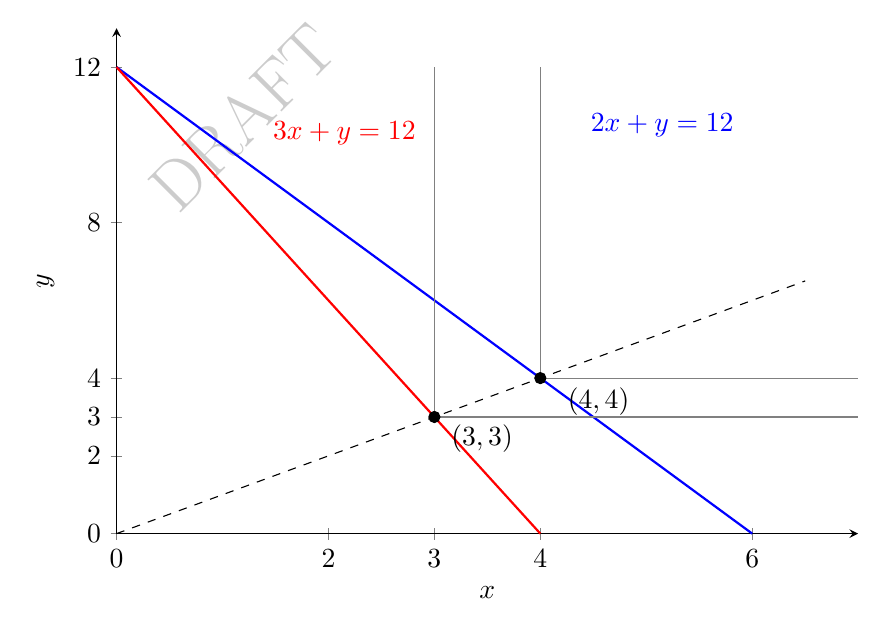
\begin{tikzpicture}
    \begin{axis}[
        width=11cm,
        height=8cm,
        xmin=0,xmax=7,
        ymin=0,ymax=13,
        axis lines=left,
        xlabel={$x$},
        ylabel={$y$},
        xtick={0,2,3,4,6},
        ytick={0,2,3,4,8,12},
        clip=false
    ]
    \addplot[domain=0:6,samples=2,thick,blue] {12-2*x};
    \addplot[domain=0:4,samples=2,thick,red] {12-3*x};
    \addplot[dashed,domain=0:6.5,samples=2,black] {x};

    \addplot[gray] coordinates {(3,12) (3,3) (7,3)};
    \addplot[gray] coordinates {(4,12) (4,4) (7,4)};

    \addplot[only marks,mark=*,mark size=2pt] coordinates {(4,4) (3,3)};

    \node[blue] at (axis cs:5.15,10.5) {$2x+y=12$};
    \node[red] at (axis cs:2.15,10.3) {$3x+y=12$};
    \node at (axis cs:4.55,3.4) {$(4,4)$};
    \node at (axis cs:3.45,2.45) {$(3,3)$};
    \end{axis}
    \end{tikzpicture}
    \end{center}
\newpage
    \item
    From part (b),
    \[
    u_1=3.
    \]
    Since \(u(x,y)=\min\{x,y\}\), attaining utility \(3\) at the original prices means choosing the kink bundle
    \[
    (x,y)=(3,3).
    \]
    At prices \((2,1)\), the required income is
    \[
    m=2(3)+1(3)=9.
    \]
    Thus the bundle is
    \[
    \boxed{(3,3)}
    \]
    and the required budget line is
    \[
    \boxed{2x+y=9}
    \qquad\text{or equivalently}\qquad
    \boxed{y=9-2x.}
    \]

    \begin{center}
    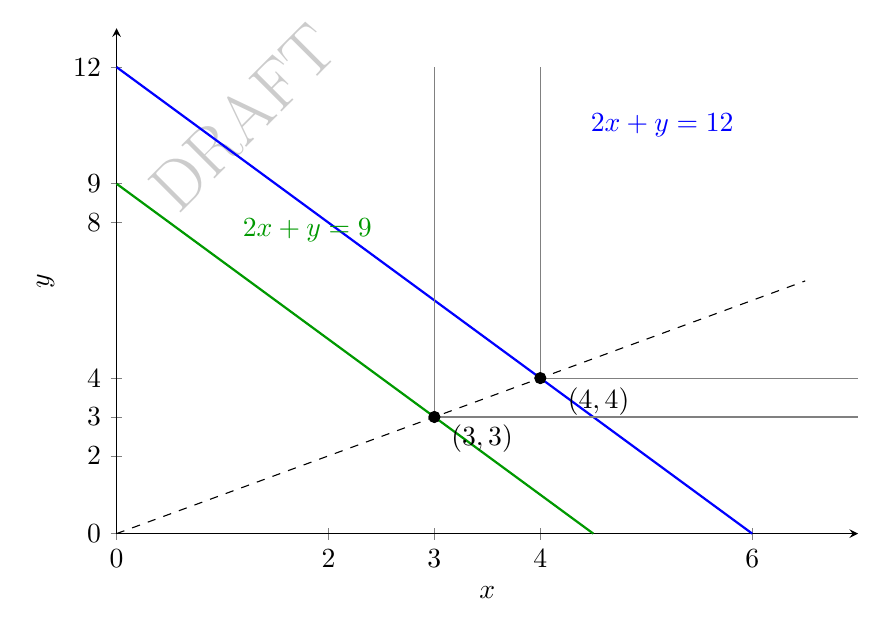
\begin{tikzpicture}
    \begin{axis}[
        width=11cm,
        height=8cm,
        xmin=0,xmax=7,
        ymin=0,ymax=13,
        axis lines=left,
        xlabel={$x$},
        ylabel={$y$},
        xtick={0,2,3,4,6},
        ytick={0,2,3,4,8,9,12},
        clip=false
    ]
    \addplot[domain=0:6,samples=2,thick,blue] {12-2*x};
    \addplot[domain=0:4.5,samples=2,thick,green!60!black] {9-2*x};
    \addplot[dashed,domain=0:6.5,samples=2,black] {x};

    \addplot[gray] coordinates {(3,12) (3,3) (7,3)};
    \addplot[gray] coordinates {(4,12) (4,4) (7,4)};

    \addplot[only marks,mark=*,mark size=2pt] coordinates {(4,4) (3,3)};

    \node[blue] at (axis cs:5.15,10.5) {$2x+y=12$};
    \node[green!60!black] at (axis cs:1.8,7.8) {$2x+y=9$};
    \node at (axis cs:4.55,3.4) {$(4,4)$};
    \node at (axis cs:3.45,2.45) {$(3,3)$};
    \end{axis}
    \end{tikzpicture}
    \end{center}

    \item
    By definition, EV is the maximum income that can be taken away at the original prices while leaving Bernice at her final utility level.
    From part (c), to attain \(u_1=3\) at the original prices, she needs income \(9\). Since her original income is \(12\),
    \[
    EV=12-9=3.
    \]
    Therefore
    \[
    \boxed{EV=3.}
    \]
\newpage
    \item
    From part (a),
    \[
    u_0=4.
    \]
    Since \(u(x,y)=\min\{x,y\}\), attaining utility \(4\) at the new prices means choosing
    \[
    (x,y)=(4,4).
    \]
    At prices \((3,1)\), the required income is
    \[
    m=3(4)+1(4)=16.
    \]
    Thus the bundle is
    \[
    \boxed{(4,4)}
    \]
    and the required budget line is
    \[
    \boxed{3x+y=16}
    \qquad\text{or equivalently}\qquad
    \boxed{y=16-3x.}
    \]

    \begin{center}
    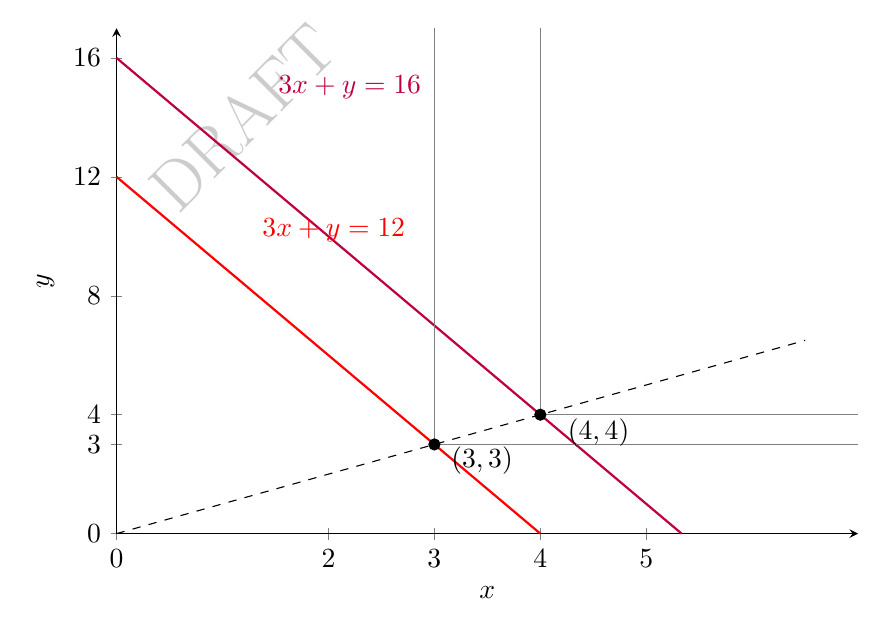
\begin{tikzpicture}
    \begin{axis}[
        width=11cm,
        height=8cm,
        xmin=0,xmax=7,
        ymin=0,ymax=17,
        axis lines=left,
        xlabel={$x$},
        ylabel={$y$},
        xtick={0,2,3,4,5},
        ytick={0,3,4,8,12,16},
        clip=false
    ]
    \addplot[domain=0:4,samples=2,thick,red] {12-3*x};
    \addplot[domain=0:5.333,samples=2,thick,purple] {16-3*x};
    \addplot[dashed,domain=0:6.5,samples=2,black] {x};

    \addplot[gray] coordinates {(3,17) (3,3) (7,3)};
    \addplot[gray] coordinates {(4,17) (4,4) (7,4)};

    \addplot[only marks,mark=*,mark size=2pt] coordinates {(3,3) (4,4)};

    \node[red] at (axis cs:2.05,10.2) {$3x+y=12$};
    \node[purple] at (axis cs:2.2,15.0) {$3x+y=16$};
    \node at (axis cs:3.45,2.45) {$(3,3)$};
    \node at (axis cs:4.55,3.4) {$(4,4)$};
    \end{axis}
    \end{tikzpicture}
    \end{center}

    \item
    By definition, CV is the least income that must be given at the new prices to restore Bernice to her original utility.
    From part (e), she needs income \(16\) at the new prices, but currently has income \(12\). Hence
    \[
    CV=16-12=4.
    \]
    Therefore
    \[
    \boxed{CV=4.}
    \]
\end{enumerate}

\newpage
\subsubsection{Method 2: Exam-style compression}
\begin{enumerate}[label=(\alph*)]
    \item
    Since \(u(x,y)=\min\{x,y\}\), Bernice chooses the kink \(x=y=u\). At the original prices,
    \[
    2x+y=12
    \;\Longrightarrow\;
    2u+u=12
    \;\Longrightarrow\;
    u_0=4.
    \]
    Hence
    \[
    \boxed{(x,y)=(4,4).}
    \]

    \item
    At the new prices,
    \[
    3x+y=12
    \;\Longrightarrow\;
    3u+u=12
    \;\Longrightarrow\;
    u_1=3.
    \]
    Hence
    \[
    \boxed{(x,y)=(3,3).}
    \]

    \item
    To attain the new utility level \(u_1=3\) at the old prices, Bernice chooses
    \[
    (3,3).
    \]
    Required income:
    \[
    m=2(3)+3=9.
    \]
    So the bundle is
    \[
    \boxed{(3,3)}
    \]
    and the budget line is
    \[
    \boxed{2x+y=9.}
    \]

    \item
    \[
    EV=12-9=3.
    \]
    Therefore
    \[
    \boxed{EV=3.}
    \]

    \item
    To attain the original utility level \(u_0=4\) at the new prices, Bernice chooses
    \[
    (4,4).
    \]
    Required income:
    \[
    m=3(4)+4=16.
    \]
    So the bundle is
    \[
    \boxed{(4,4)}
    \]
    and the budget line is
    \[
    \boxed{3x+y=16.}
    \]

    \item
    \[
    CV=16-12=4.
    \]
    Therefore
    \[
    \boxed{CV=4.}
    \]
\end{enumerate}

\newpage
\subsubsection{Method 3: Duality / expenditure and Hicksian demand}
\begin{enumerate}[label=(\alph*)]
    \item
    For \(u(x,y)=\min\{x,y\}\), the Hicksian problem is
    \[
    \min_{x,y}\; p_xx+p_yy
    \quad\text{subject to}\quad
    \min\{x,y\}\ge u.
    \]
    The constraint is equivalent to
    \[
    x\ge u,\qquad y\ge u,
    \]
    so cost minimisation gives
    \[
    h_x(p,u)=u,\qquad h_y(p,u)=u.
    \]
    Hence the expenditure function is
    \[
    e((p_x,p_y),u)=p_xu+p_yu=(p_x+p_y)u.
    \]
    At prices \((2,1)\),
    \[
    e((2,1),u)=3u.
    \]
    Since income is \(12\),
    \[
    3u=12
    \;\Longrightarrow\;
    u_0=4.
    \]
    Therefore the optimal bundle is
    \[
    \boxed{(4,4)}.
    \]

    \item
    At the new prices \((3,1)\),
    \[
    e((3,1),u)=4u.
    \]
    Since income is still \(12\),
    \[
    4u=12
    \;\Longrightarrow\;
    u_1=3.
    \]
    Therefore the new optimal bundle is
    \[
    \boxed{(3,3)}.
    \]

    \item
    To attain \(u_1=3\) at the old prices,
    \[
    e((2,1),3)=3\cdot 3=9.
    \]
    Thus the required bundle is
    \[
    \boxed{(3,3)}
    \]
    and the budget line is
    \[
    \boxed{2x+y=9.}
    \]

    \item
    By definition,
    \[
    EV=m-e(p_0,u_1).
    \]
    Here \(m=12\), \(p_0=(2,1)\), and \(u_1=3\). Hence
    \[
    EV=12-e((2,1),3)=12-9=3.
    \]
    Therefore
    \[
    \boxed{EV=3.}
    \]

    \item
    To attain \(u_0=4\) at the new prices,
    \[
    e((3,1),4)=4\cdot 4=16.
    \]
    Thus the required bundle is
    \[
    \boxed{(4,4)}
    \]
    and the budget line is
    \[
    \boxed{3x+y=16.}
    \]

    \item
    By definition,
    \[
    CV=e(p_1,u_0)-m.
    \]
    Here \(p_1=(3,1)\), \(u_0=4\), and \(m=12\). Hence
    \[
    CV=e((3,1),4)-12=16-12=4.
    \]
    Therefore
    \[
    \boxed{CV=4.}
    \]
\end{enumerate}

%====================================================
% QUESTION 2
%====================================================
\newpage
\section{Question 2: Steve, Reservation Prices, and Inverse Demand}

\noindent
Steve consumes earplugs and other goods. His utility function \(U(x,y)\) is increasing in both his consumption of earplugs \(x\) and other goods \(y\). Suppose that Steve has a sufficiently large income \(I\).

\subsection{Problem}
\begin{enumerate}[label=(\alph*)]
    \item Suppose \(U(x,y)=v(x)+ay\) and that Steve can buy \(n-1\) units of earplugs at total cost \(c_{n-1}\).
    \begin{enumerate}[label=(\roman*)]
        \item Write out Steve’s utility of consuming \(n-1\) units of earplugs and spending the rest on other goods.
        \item Suppose that the \(n\)th earplug costs \(p_n\), write out Steve’s utility of consuming \(n\) units of earplugs and spending the rest on other goods.
        \item Show that the reservation price for the \(n\)th earplug \(r_n\) is \(\dfrac{p_y}{a}\times [v(n)-v(n-1)]\).

        (Hint: look at the definition of the reservation price.)

        Note that this implies that if earplugs were perfectly divisible, the reservation price function \(r(n)=\dfrac{p_y}{a}v'(n)\).
    \end{enumerate}
    \item Solve Steve’s utility maximisation problem (subject to prices \(p_x,p_y\) and wealth \(w\)) to get his inverse demand function for earplugs \(x\). Is it the same as the reservation price function?
    \item In the lecture’s example, \(a=1\) and \(p_y=1\) such that the reservation price curve is \(p_x=v'(x)\). What do you think the additional term \(\dfrac{p_y}{a}\) captures?
\end{enumerate}

\newpage
\subsection{Solution}

\subsubsection{Method 1: Direct utility comparisons and optimisation}
\begin{enumerate}[label=(\alph*)]
    \item
    \begin{enumerate}[label=(\roman*)]
        \item
        Since
        \[
        U(x,y)=v(x)+ay,
        \]
        if Steve consumes \(n-1\) earplugs and total spending on those earplugs is \(c_{n-1}\), then he has
        \[
        I-c_{n-1}
        \]
        dollars left for the other good. Since the other good costs \(p_y\) per unit, he buys
        \[
        y=\frac{I-c_{n-1}}{p_y}
        \]
        units of it. Therefore his utility is
        \[
        U_{n-1}=v(n-1)+a\left(\frac{I-c_{n-1}}{p_y}\right).
        \]
        Hence
        \[
        \boxed{\,U_{n-1}=v(n-1)+\frac{a}{p_y}(I-c_{n-1})\,.}
        \]

        \item
        If the \(n\)th earplug costs \(p_n\), then total spending on earplugs becomes
        \[
        c_{n-1}+p_n,
        \]
        so the remaining money is
        \[
        I-c_{n-1}-p_n.
        \]
        Hence Steve buys
        \[
        y=\frac{I-c_{n-1}-p_n}{p_y}
        \]
        units of the other good, and his utility becomes
        \[
        U_n=v(n)+a\left(\frac{I-c_{n-1}-p_n}{p_y}\right).
        \]
        Therefore
        \[
        \boxed{\,U_n=v(n)+\frac{a}{p_y}(I-c_{n-1}-p_n)\,.}
        \]
\newpage
        \item
        By definition, the reservation price \(r_n\) is the price that makes Steve indifferent between consuming \(n-1\) earplugs and consuming \(n\) earplugs. Therefore
        \[
        v(n-1)+\frac{a}{p_y}(I-c_{n-1})
        =
        v(n)+\frac{a}{p_y}(I-c_{n-1}-r_n).
        \]
        Cancelling the common term \(\frac{a}{p_y}(I-c_{n-1})\),
        \[
        v(n-1)=v(n)-\frac{a}{p_y}r_n.
        \]
        Rearranging gives
        \[
        \frac{a}{p_y}r_n=v(n)-v(n-1),
        \]
        so
        \[
        \boxed{\,r_n=\frac{p_y}{a}[v(n)-v(n-1)]\,.}
        \]
        In the perfectly divisible case, the finite difference becomes a derivative, so
        \[
        \boxed{\,r(x)=\frac{p_y}{a}v'(x)\,.}
        \]
    \end{enumerate}

    \item
    Steve solves
    \[
    \max_{x,y}\; v(x)+ay
    \quad\text{subject to}\quad
    p_xx+p_yy=w.
    \]
    Substitute
    \[
    y=\frac{w-p_xx}{p_y}
    \]
    into utility:
    \[
    U(x)=v(x)+a\left(\frac{w-p_xx}{p_y}\right)
    =v(x)+\frac{aw}{p_y}-\frac{ap_x}{p_y}x.
    \]
    Since \(\frac{aw}{p_y}\) is constant, Steve equivalently solves
    \[
    \max_x\; v(x)-\frac{ap_x}{p_y}x.
    \]
    The first-order condition is
    \[
    v'(x)-\frac{ap_x}{p_y}=0.
    \]
    Hence
    \[
    p_x=\frac{p_y}{a}v'(x).
    \]
    Therefore Steve’s inverse demand function is
    \[
    \boxed{\,p_x=\frac{p_y}{a}v'(x)\,.}
    \]

    It is not literally the same as the discrete reservation-price formula
    \[
    r_n=\frac{p_y}{a}[v(n)-v(n-1)],
    \]
    because that uses a finite difference, whereas inverse demand uses a derivative. However, in the perfectly divisible case the reservation-price function becomes
    \[
    r(x)=\frac{p_y}{a}v'(x),
    \]
    so the two coincide in the continuous formulation.

    \item
    The factor
    \[
    \frac{p_y}{a}
    \]
    converts utility units into money units. One unit of the other good costs \(p_y\) dollars and contributes \(a\) units of utility, so one util corresponds to
    \[
    \frac{p_y}{a}
    \]
    dollars’ worth of the other good. Thus \(\frac{p_y}{a}\) measures the money value of one util, using the outside good as the benchmark.

    Therefore
    \[
    \boxed{\,\frac{p_y}{a}\text{ is the utility-to-money conversion factor.}\,}
    \]
\end{enumerate}

\newpage
\subsubsection{Method 2: Utility function method}
\begin{enumerate}[label=(\alph*)]
    \item
    \begin{enumerate}[label=(\roman*)]
        \item
        \[
        U_{n-1}=v(n-1)+a\left(\frac{I-c_{n-1}}{p_y}\right)
        =\boxed{\,v(n-1)+\frac{a}{p_y}(I-c_{n-1})\, }.
        \]

        \item
        \[
        U_n=v(n)+a\left(\frac{I-c_{n-1}-p_n}{p_y}\right)
        =\boxed{\,v(n)+\frac{a}{p_y}(I-c_{n-1}-p_n)\, }.
        \]

        \item
        Reservation price means indifference:
        \[
        v(n-1)+\frac{a}{p_y}(I-c_{n-1})
        =
        v(n)+\frac{a}{p_y}(I-c_{n-1}-r_n).
        \]
        Hence
        \[
        \boxed{\,r_n=\frac{p_y}{a}[v(n)-v(n-1)]\, }.
        \]
        If earplugs are perfectly divisible,
        \[
        \boxed{\,r(x)=\frac{p_y}{a}v'(x)\, }.
        \]
    \end{enumerate}

    \item
    \[
    \max_{x,y}\; v(x)+ay
    \quad\text{s.t.}\quad
    p_xx+p_yy=w.
    \]
    Substitute \(y=(w-p_xx)/p_y\):
    \[
    \max_x\; v(x)-\frac{ap_x}{p_y}x.
    \]
    FOC:
    \[
    v'(x)=\frac{ap_x}{p_y}.
    \]
    Therefore
    \[
    \boxed{\,p_x=\frac{p_y}{a}v'(x)\, }.
    \]
    This matches the reservation-price function only in the perfectly divisible case.

    \item
    \[
    \boxed{\,\frac{p_y}{a}\text{ converts utils into dollars via the outside good.}\,}
    \]
\end{enumerate}

\newpage
\subsubsection{Method 3: Indirect-utility / envelope viewpoint}
\begin{enumerate}[label=(\alph*)]
    \item
    \begin{enumerate}[label=(\roman*)]
        \item
        \[
        \boxed{\,U_{n-1}=v(n-1)+\frac{a}{p_y}(I-c_{n-1})\, }.
        \]

        \item
        \[
        \boxed{\,U_n=v(n)+\frac{a}{p_y}(I-c_{n-1}-p_n)\, }.
        \]

        \item
        Reservation price is the price that leaves utility unchanged, so
        \[
        \boxed{\,r_n=\frac{p_y}{a}[v(n)-v(n-1)]\, }.
        \]
    \end{enumerate}

    \item
    Define the indirect objective
    \[
    \Phi(x;p_x,p_y,w)=v(x)+a\frac{w-p_xx}{p_y}.
    \]
    Then indirect utility is
    \[
    V(p_x,p_y,w)=\max_x \Phi(x;p_x,p_y,w).
    \]
    The optimiser \(x^*\) satisfies
    \[
    \frac{\partial \Phi}{\partial x}=v'(x)-\frac{ap_x}{p_y}=0.
    \]
    Hence
    \[
    \boxed{\,p_x=\frac{p_y}{a}v'(x)\, }.
    \]
    Because wealth enters only through the additive term \(aw/p_y\), earplug demand has no income effect in the interior solution.

    \item
    Since \(y\) is quasi-linear,
    \[
    U(x,y)=v(x)+ay,
    \]
    the outside good acts as the numeraire benchmark for utility. Therefore
    \[
    \boxed{\,\frac{p_y}{a}\text{ captures the dollar value of one unit of utility relative to the outside good.}\,}
    \]
\end{enumerate}

%====================================================
% QUESTION 3
%====================================================
\newpage
%====================================================

\section{Question 3: Lolita, EV, CV, and Consumer Surplus}

\noindent
Lolita, an intelligent and charming Holstein cow, consumes only two goods, cow feed (made of ground corn and oats) and hay. Her preferences are represented by the utility function
\[
U(x,y)=x-\frac{x^2}{2}+y,
\]
where \(x\) is her consumption of cow feed and \(y\) is her consumption of hay. Lolita has been instructed in the mysteries of budgets and optimization and always maximizes her utility subject to her budget constraint. Lolita has an income of \(\$ I\) that she is allowed to spend as she wishes on cow feed and hay. The price of hay is always \(\$1\), and the price of cow feed will be denoted by \(p\), where \(0<p\le 1\).

\subsection{Problem}
\begin{enumerate}[label=(\alph*)]
    \item Write Lolita’s demand function for cow feed and hay as a function of \(I\) and \(p\).
    \item Write out the indirect utility function of Lolita at income \(I\) and prices \(p\). (Remember that indirect utility is the maximum level of utility that she enjoys at this price and income.)
\end{enumerate}

\noindent
Suppose that Lolita’s daily income is \(\$3\) and that the price of feed is \(\$0.50\). There is a price increase from \(\$0.50\) to \(\$1\) for cow feed.

\begin{enumerate}[label=(\alph*),start=3]
    \item Consider the largest fee Lolita is willing to pay to avoid having the price of cow feed rise to \(\$1\). Is this EV or CV?
    \item Consider the extra money would you have to pay Lolita to make her as well-off as she was at the old prices. Is this EV or CV?
    \item Use the indirect utility function to calculate Lolita’s CV and EV.
    \item What is the change in consumer surplus of the price increase of cow feed from \(\$0.5\) to \(\$1\)?
\end{enumerate}

\newpage
\subsection{Solution}

\subsubsection{Method 1: Direct optimisation and triangle-surplus method}
\begin{enumerate}[label=(\alph*)]
    \item
    Lolita solves
    \[
    \max_{x,y}\; x-\frac{x^2}{2}+y
    \qquad\text{subject to}\qquad
    px+y=I,
    \]
    with \(x\ge 0\), \(y\ge 0\). Substituting
    \[
    y=I-px
    \]
    into utility gives the one-variable problem
    \[
    \max_{0\le x\le I/p}\;
    I+(1-p)x-\frac{x^2}{2}.
    \]
    Since
    \[
    \frac{d^2}{dx^2}\!\left(I+(1-p)x-\frac{x^2}{2}\right)=-1<0,
    \]
    the objective is strictly concave, so the unconstrained maximiser is given by
    \[
    (1-p)-x=0
    \quad\Longrightarrow\quad
    x=1-p.
    \]
    Hence the demand for cow feed is
    \[
    x^*(I,p)=\min\left\{1-p,\frac{I}{p}\right\},
    \]
    and the demand for hay is
    \[
    y^*(I,p)=I-p\,x^*(I,p).
    \]
    Therefore
    \[
    \boxed{\;
    x^*(I,p)=\min\left\{1-p,\frac{I}{p}\right\},
    \qquad
    y^*(I,p)=I-p\min\left\{1-p,\frac{I}{p}\right\}.
    \;}
    \]

    \item
    Using the demand found in part (a), the indirect utility is
    \[
    V(I,p)=\max_{0\le x\le I/p}\left\{I+(1-p)x-\frac{x^2}{2}\right\}.
    \]
    There are two cases.

    If \(1-p\le I/p\), then the interior optimum is feasible and
    \[
    x^*=1-p,
    \qquad
    y^*=I-p(1-p).
    \]
    Hence
    \[
    V(I,p)
    =
    (1-p)-\frac{(1-p)^2}{2}+I-p(1-p)
    =
    I+\frac{(1-p)^2}{2}.
    \]

    If \(1-p>I/p\), then the optimum is at the boundary \(x^*=I/p\), \(y^*=0\), so
    \[
    V(I,p)
    =
    \frac{I}{p}-\frac{1}{2}\left(\frac{I}{p}\right)^2.
    \]

    Therefore
    \[
    \boxed{
    V(I,p)=
    \begin{cases}
    I+\dfrac{(1-p)^2}{2}, & \text{if } 1-p\le \dfrac{I}{p},\\[1.2ex]
    \dfrac{I}{p}-\dfrac{1}{2}\left(\dfrac{I}{p}\right)^2, & \text{if } 1-p>\dfrac{I}{p}.
    \end{cases}}
    \]

    \item
    The largest fee Lolita is willing to pay \emph{to avoid} the price rise is the amount that can be taken away \emph{at the old prices} while leaving her at the same utility as after the price increase. That is exactly the \emph{equivalent variation}.

    Hence
    \[
    \boxed{\text{This is EV.}}
    \]

    \item
    The extra money that must be given to Lolita \emph{at the new prices} to make her as well-off as she was at the old prices is, by definition, the \emph{compensating variation}.

    Hence
    \[
    \boxed{\text{This is CV.}}
    \]

    \item
    Here \(I=3\), initially \(p_0=0.5\), and finally \(p_1=1\). Since
    \[
    1-p_0=0.5\le \frac{3}{0.5}=6,
    \qquad
    1-p_1=0\le \frac{3}{1}=3,
    \]
    both situations lie in the interior branch of \(V\). Thus
    \[
    V(3,0.5)=3+\frac{(1-0.5)^2}{2}
    =3+\frac{(0.5)^2}{2}
    =3+\frac18
    =\frac{25}{8},
    \]
    and
    \[
    V(3,1)=3+\frac{(1-1)^2}{2}=3.
    \]

    For EV, let \(m^{EV}\) be the income at old prices \(p_0=0.5\) that gives final utility \(3\):
    \[
    V(m^{EV},0.5)=3.
    \]
    Since we remain on the interior branch,
    \[
    m^{EV}+\frac18=3
    \quad\Longrightarrow\quad
    m^{EV}=\frac{23}{8}.
    \]
    Hence
    \[
    EV=3-\frac{23}{8}=\frac18.
    \]

    For CV, let \(m^{CV}\) be the income at new prices \(p_1=1\) that gives initial utility \(25/8\):
    \[
    V(m^{CV},1)=\frac{25}{8}.
    \]
    Since \(V(m,1)=m\),
    \[
    m^{CV}=\frac{25}{8}.
    \]
    Hence
    \[
    CV=\frac{25}{8}-3=\frac18.
    \]

    Therefore
    \[
    \boxed{EV=\frac18,\qquad CV=\frac18.}
    \]

    \item
    From part (a), for \(0<p\le 1\) and with income large enough for the interior solution,
    \[
    x=1-p.
    \]
    So the inverse demand curve is
    \[
    p=1-x.
    \]
    When price rises from \(0.5\) to \(1\), quantity falls from
    \[
    x_0=1-0.5=0.5
    \qquad\text{to}\qquad
    x_1=1-1=0.
    \]
    The lost consumer surplus is the area of the triangle under inverse demand and above the new price line between \(x=0\) and \(x=0.5\):
    \[
    \frac12 \times 0.5 \times 0.5=\frac18.
    \]
    Since the question asks for the \emph{change} in consumer surplus,
    \[
    \Delta CS=CS_{\text{new}}-CS_{\text{old}}=-\frac18.
    \]

    Therefore
    \[
    \boxed{\Delta CS=-\frac18.}
    \]
\end{enumerate}

\newpage
\subsubsection{Method 2: Quasilinear welfare shortcut and integration method}
\begin{enumerate}[label=(\alph*)]
    \item
    With
    \[
    U(x,y)=\phi(x)+y,
    \qquad
    \phi(x)=x-\frac{x^2}{2},
    \]
    the problem is quasilinear in \(y\). Substituting \(y=I-px\), Lolita solves
    \[
    \max_{0\le x\le I/p}\;\phi(x)-px+I.
    \]
    Since
    \[
    \phi'(x)=1-x,
    \]
    the interior first-order condition is
    \[
    \phi'(x)=p
    \quad\Longleftrightarrow\quad
    1-x=p
    \quad\Longleftrightarrow\quad
    x=1-p.
    \]
    Hence
    \[
    \boxed{
    x^*(I,p)=\min\left\{1-p,\frac{I}{p}\right\},
    \qquad
    y^*(I,p)=I-p\,x^*(I,p).
    }
    \]

    \item
    The indirect utility is
    \[
    V(I,p)=I+\max_{0\le x\le I/p}\left\{\phi(x)-px\right\}.
    \]
    If \(1-p\le I/p\), then the interior maximiser is feasible and
    \[
    V(I,p)=I+\phi(1-p)-p(1-p).
    \]
    Since
    \[
    \phi(1-p)=(1-p)-\frac{(1-p)^2}{2},
    \]
    this becomes
    \[
    V(I,p)=I+\frac{(1-p)^2}{2}.
    \]
    If \(1-p>I/p\), then \(x^*=I/p\), so
    \[
    V(I,p)=I+\phi\!\left(\frac{I}{p}\right)-p\left(\frac{I}{p}\right)
    =\frac{I}{p}-\frac12\left(\frac{I}{p}\right)^2.
    \]
    Therefore
    \[
    \boxed{
    V(I,p)=
    \begin{cases}
    I+\dfrac{(1-p)^2}{2}, & \text{if } 1-p\le \dfrac{I}{p},\\[1.2ex]
    \dfrac{I}{p}-\dfrac12\left(\dfrac{I}{p}\right)^2, & \text{if } 1-p>\dfrac{I}{p}.
    \end{cases}}
    \]

\newpage
    \item
    The largest fee Lolita is willing to pay \emph{at the old prices} to avoid the price increase is
    \[
    \boxed{\text{EV}.}
    \]

    \item
    The extra money needed \emph{at the new prices} to restore old utility is
    \[
    \boxed{\text{CV}.}
    \]

    \item
    Since \(I=3\) is sufficiently large here, demand remains on the quasilinear interior branch:
    \[
    x(p)=1-p,\qquad 0<p\le 1.
    \]
    Therefore the welfare loss from the price increase from \(p_0=0.5\) to \(p_1=1\) is
    \[
    \int_{p_0}^{p_1} x(p)\,dp
    =
    \int_{0.5}^{1}(1-p)\,dp
    =
    \left[p-\frac{p^2}{2}\right]_{0.5}^{1}
    =
    \frac18.
    \]
    For quasilinear preferences, the welfare loss equals both EV and CV. Hence
    \[
    \boxed{EV=\frac18,\qquad CV=\frac18.}
    \]

    \item
    The change in consumer surplus is
    \[
    \Delta CS
    =
    -\int_{0.5}^{1}x(p)\,dp
    =
    -\int_{0.5}^{1}(1-p)\,dp
    =
    -\frac18.
    \]
    Therefore
    \[
    \boxed{\Delta CS=-\frac18.}
    \]
\end{enumerate}

\newpage
\subsubsection{Method 3: Duality method}
\begin{enumerate}[label=(\alph*)]
    \item
    For fixed \(I\) and \(p\), the Marshallian problem is
    \[
    \max_{x,y}\; x-\frac{x^2}{2}+y
    \qquad\text{s.t.}\qquad
    px+y=I.
    \]
    Since utility is quasilinear, it is convenient to isolate the non-numeraire part. Define
    \[
    \phi(x)=x-\frac{x^2}{2}.
    \]
    Then
    \[
    U(x,y)=\phi(x)+y.
    \]
    The optimal \(x\) solves
    \[
    \max_{0\le x\le I/p}\{\phi(x)-px\}.
    \]
    The first-order condition for an interior maximiser is
    \[
    \phi'(x)=p
    \quad\Longleftrightarrow\quad
    1-x=p
    \quad\Longleftrightarrow\quad
    x=1-p.
    \]
    Hence
    \[
    \boxed{
    x^*(I,p)=\min\left\{1-p,\frac{I}{p}\right\},
    \qquad
    y^*(I,p)=I-p\,x^*(I,p).
    }
    \]

    \item
    The expenditure function at utility level \(u\) is
    \[
    e(p,u)=\min_x\{px+u-\phi(x)\}
    =
    u+\min_x\{px-\phi(x)\}.
    \]
    Equivalently,
    \[
    e(p,u)=u-\max_x\{\phi(x)-px\}.
    \]
    For \(0<p\le 1\), the maximiser of \(\phi(x)-px\) is \(x=1-p\), so
    \[
    \max_x\{\phi(x)-px\}
    =
    \phi(1-p)-p(1-p)
    =
    \frac{(1-p)^2}{2}.
    \]
    Therefore
    \[
    e(p,u)=u-\frac{(1-p)^2}{2}.
    \]
    Using the dual identity
    \[
    V(I,p)=\max\{u:e(p,u)\le I\},
    \]
    we obtain
    \[
    I=e(p,u)
    =u-\frac{(1-p)^2}{2}
    \quad\Longrightarrow\quad
    u=I+\frac{(1-p)^2}{2},
    \]
    whenever the interior solution applies. Thus
    \[
    \boxed{
    V(I,p)=I+\frac{(1-p)^2}{2}
    }
    \]
    on the relevant branch, and together with the boundary case this yields
    \[
    \boxed{
    V(I,p)=
    \begin{cases}
    I+\dfrac{(1-p)^2}{2}, & \text{if } 1-p\le \dfrac{I}{p},\\[1.2ex]
    \dfrac{I}{p}-\dfrac12\left(\dfrac{I}{p}\right)^2, & \text{if } 1-p>\dfrac{I}{p}.
    \end{cases}}
    \]

    \item
    The largest fee paid at old prices to avoid the price increase is
    \[
    \boxed{\text{EV}.}
    \]

    \item
    The extra money required at new prices to restore the old utility is
    \[
    \boxed{\text{CV}.}
    \]

    \item
    At \(I=3\), both \(p_0=0.5\) and \(p_1=1\) lie on the interior branch. Hence
    \[
    V(3,0.5)=3+\frac{(0.5)^2}{2}=\frac{25}{8},
    \qquad
    V(3,1)=3.
    \]
    From the expenditure function,
    \[
    e(p,u)=u-\frac{(1-p)^2}{2}.
    \]
    Therefore
    \[
    EV
    =
    I-e(p_0,V(3,p_1))
    =
    3-e(0.5,3)
    =
    3-\left(3-\frac18\right)
    =
    \frac18,
    \]
    and
    \[
    CV
    =
    e(p_1,V(3,p_0))-I
    =
    e\!\left(1,\frac{25}{8}\right)-3
    =
    \frac{25}{8}-3
    =
    \frac18.
    \]
    Thus
    \[
    \boxed{EV=\frac18,\qquad CV=\frac18.}
    \]

    \item
    Since quasilinearity implies
    \[
    \max_x\{\phi(x)-px\}=\frac{(1-p)^2}{2},
    \]
    the surplus loss from \(p_0=0.5\) to \(p_1=1\) is
    \[
    \frac{(1-0.5)^2}{2}-\frac{(1-1)^2}{2}
    =\frac18.
    \]
    Hence the change in consumer surplus is
    \[
    \boxed{\Delta CS=-\frac18.}
    \]
\end{enumerate}

\newpage
\subsubsection{Method 4: Legendre-transform method}
\begin{enumerate}[label=(\alph*)]
    \item
    Let
    \[
    \phi(x)=x-\frac{x^2}{2}.
    \]
    The indirect problem is
    \[
    V(I,p)
    =
    I+\sup_{0\le x\le I/p}\{\phi(x)-px\}.
    \]
    On the interior region, the supremum is attained where
    \[
    \phi'(x)=p
    \quad\Longleftrightarrow\quad
    1-x=p
    \quad\Longleftrightarrow\quad
    x=1-p.
    \]
    Hence
    \[
    \boxed{
    x^*(I,p)=\min\left\{1-p,\frac{I}{p}\right\},
    \qquad
    y^*(I,p)=I-p\,x^*(I,p).
    }
    \]

    \item
    The Legendre transform of \(\phi\) at slope \(p\) is
    \[
    \phi^*(p):=\sup_x\{\phi(x)-px\}.
    \]
    For \(0<p\le 1\), the maximiser is \(x=1-p\), so
    \[
    \phi^*(p)
    =
    \left(1-p\right)-\frac{(1-p)^2}{2}-p(1-p)
    =
    \frac{(1-p)^2}{2}.
    \]
    Therefore, on the interior branch,
    \[
    V(I,p)=I+\phi^*(p)=I+\frac{(1-p)^2}{2}.
    \]
    Including the boundary branch,
    \[
    \boxed{
    V(I,p)=
    \begin{cases}
    I+\dfrac{(1-p)^2}{2}, & \text{if } 1-p\le \dfrac{I}{p},\\[1.2ex]
    \dfrac{I}{p}-\dfrac12\left(\dfrac{I}{p}\right)^2, & \text{if } 1-p>\dfrac{I}{p}.
    \end{cases}}
    \]

    \item
    The largest fee paid at old prices to avoid the price increase is
    \[
    \boxed{\text{EV}.}
    \]

    \item
    The extra money needed at new prices to restore old utility is
    \[
    \boxed{\text{CV}.}
    \]

    \item
    Since \(I=3\) is large relative to both prices, the relevant formula is
    \[
    V(I,p)=I+\phi^*(p)=I+\frac{(1-p)^2}{2}.
    \]
    Thus
    \[
    V(3,0.5)=3+\phi^*(0.5)=3+\frac18=\frac{25}{8},
    \qquad
    V(3,1)=3+\phi^*(1)=3.
    \]
    Hence
    \[
    EV=\phi^*(0.5)-\phi^*(1)=\frac18,
    \qquad
    CV=\phi^*(0.5)-\phi^*(1)=\frac18.
    \]
    Therefore
    \[
    \boxed{EV=\frac18,\qquad CV=\frac18.}
    \]

    \item
    Consumer surplus change equals the change in the conjugate surplus term:
    \[
    \Delta CS
    =
    \phi^*(1)-\phi^*(0.5)
    =
    0-\frac18
    =
    -\frac18.
    \]
    Therefore
    \[
    \boxed{\Delta CS=-\frac18.}
    \]
\end{enumerate}

%====================================================
% QUESTION 4
%====================================================
\newpage
%====================================================
% QUESTION 4
%====================================================
\newpage
\section{Question 4: Cobb Douglas Utility and Cost Minimisation}

\noindent
Consider a consumer with cobb douglas utility
\[
U(x_1,x_2)=x_1^{0.4}x_2^{0.6}.
\]

\subsection{Problem}
\begin{enumerate}[label=(\alph*)]
    \item Derive the demand functions for \(x_1\) and \(x_2\) for prices \(p_1,p_2\) and income \(I\).
    \item Derive the consumer’s indirect utility function.
\end{enumerate}

\noindent
Consider initial prices \(p_1=10,p_2=10\). The price of good \(2\) increases from \(10\) to \(20\). Income remains fixed at \(I=100\).

\begin{enumerate}[label=(\alph*),start=3]
    \item What is the consumer’s maximum utility at the initial prices.
    \item * What is the lowest cost consumption bundle \((x_1,x_2)\) which at the new prices, gives the consumer the utility in (c)?
\end{enumerate}

\subsection{Solution}

\subsubsection{Method 1: Direct optimisation and Hicksian reconstruction}
\begin{enumerate}[label=(\alph*)]
    \item
    The consumer solves
    \[
    \max_{x_1,x_2>0}\; x_1^{0.4}x_2^{0.6}
    \qquad\text{subject to}\qquad
    p_1x_1+p_2x_2=I.
    \]
    Form the Lagrangian
    \[
    \mathcal L=x_1^{0.4}x_2^{0.6}+\lambda(I-p_1x_1-p_2x_2).
    \]
    The first-order conditions are
    \[
    0.4x_1^{-0.6}x_2^{0.6}=\lambda p_1,
    \qquad
    0.6x_1^{0.4}x_2^{-0.4}=\lambda p_2.
    \]
    Dividing the first equation by the second gives
    \[
    \frac{0.4}{0.6}\frac{x_2}{x_1}=\frac{p_1}{p_2},
    \]
    so
    \[
    \frac{2}{3}\frac{x_2}{x_1}=\frac{p_1}{p_2}
    \quad\Longrightarrow\quad
    x_2=\frac{3p_1}{2p_2}x_1.
    \]
    Substitute into the budget constraint:
    \[
    p_1x_1+p_2\left(\frac{3p_1}{2p_2}x_1\right)=I
    \quad\Longrightarrow\quad
    \frac{5}{2}p_1x_1=I.
    \]
    Hence
    \[
    x_1^*(p_1,p_2,I)=\frac{2I}{5p_1}=\frac{0.4I}{p_1}.
    \]
    Then
    \[
    x_2^*(p_1,p_2,I)=\frac{I-p_1x_1^*}{p_2}
    =\frac{I-0.4I}{p_2}
    =\frac{0.6I}{p_2}.
    \]
    Therefore
    \[
    \boxed{
    x_1^*(p_1,p_2,I)=\frac{0.4I}{p_1},
    \qquad
    x_2^*(p_1,p_2,I)=\frac{0.6I}{p_2}.
    }
    \]

    \item
    Substitute the Marshallian demands into utility:
    \[
    V(p_1,p_2,I)
    =
    \left(\frac{0.4I}{p_1}\right)^{0.4}
    \left(\frac{0.6I}{p_2}\right)^{0.6}.
    \]
    Hence
    \[
    \boxed{
    V(p_1,p_2,I)
    =
    0.4^{0.4}0.6^{0.6}\,
    I\,
    p_1^{-0.4}p_2^{-0.6}.
    }
    \]

    \item
    At the initial prices \(p_1=p_2=10\) and income \(I=100\),
    \[
    x_1^*=\frac{0.4(100)}{10}=4,
    \qquad
    x_2^*=\frac{0.6(100)}{10}=6.
    \]
    Therefore the maximum utility is
    \[
    u_0=4^{0.4}6^{0.6}.
    \]

    Hence
    \[
    \boxed{u_0=4^{0.4}6^{0.6}\approx 5.101698.}
    \]

    \item
    Now prices are \(p_1=10\), \(p_2=20\). We seek the expenditure-minimising bundle that attains utility \(u_0\). Thus solve
    \[
    \min_{x_1,x_2>0}\;10x_1+20x_2
    \qquad\text{subject to}\qquad
    x_1^{0.4}x_2^{0.6}=u_0.
    \]
    At an interior Hicksian optimum,
    \[
    \frac{MU_1}{MU_2}=\frac{p_1}{p_2}.
    \]
    Since
    \[
    MU_1=0.4x_1^{-0.6}x_2^{0.6},
    \qquad
    MU_2=0.6x_1^{0.4}x_2^{-0.4},
    \]
    this gives
    \[
    \frac{0.4}{0.6}\frac{x_2}{x_1}=\frac{10}{20}=\frac12.
    \]
    Hence
    \[
    \frac{2}{3}\frac{x_2}{x_1}=\frac12
    \quad\Longrightarrow\quad
    \frac{x_2}{x_1}=\frac34
    \quad\Longrightarrow\quad
    x_2=\frac34x_1.
    \]
    Impose the utility constraint:
    \[
    x_1^{0.4}\left(\frac34x_1\right)^{0.6}=u_0
    \quad\Longrightarrow\quad
    x_1\left(\frac34\right)^{0.6}=u_0.
    \]
    Therefore
    \[
    x_1=u_0\left(\frac43\right)^{0.6}.
    \]
    Since
    \[
    u_0=4^{0.4}6^{0.6},
    \]
    we get
    \[
    x_1
    =
    4^{0.4}6^{0.6}\left(\frac43\right)^{0.6}
    =
    4^{0.4}8^{0.6}
    =
    4\cdot 2^{0.6}
    =
    4\cdot 2^{3/5}.
    \]
    Thus
    \[
    x_2=\frac34x_1=3\cdot 2^{3/5}.
    \]
    Numerically,
    \[
    x_1\approx 6.062866,
    \qquad
    x_2\approx 4.547150.
    \]
    Therefore the lowest-cost bundle is
    \[
    \boxed{\left(x_1,x_2\right)=\left(4\cdot 2^{3/5},\,3\cdot 2^{3/5}\right)\approx(6.062866,\,4.547150).}
    \]
\end{enumerate}

\newpage
\subsubsection{Method 2: Expenditure-share and expenditure-function method}
\begin{enumerate}[label=(\alph*)]
    \item
    For Cobb Douglas utility \(x_1^{0.4}x_2^{0.6}\), the Marshallian demands allocate fixed expenditure shares:
    \[
    40\%\text{ of income to good }1,
    \qquad
    60\%\text{ of income to good }2.
    \]
    Hence
    \[
    \boxed{
    x_1^*(p_1,p_2,I)=\frac{0.4I}{p_1},
    \qquad
    x_2^*(p_1,p_2,I)=\frac{0.6I}{p_2}.
    }
    \]

    \item
    Substituting these into utility,
    \[
    V(p_1,p_2,I)
    =
    \left(\frac{0.4I}{p_1}\right)^{0.4}
    \left(\frac{0.6I}{p_2}\right)^{0.6}.
    \]
    Therefore
    \[
    \boxed{
    V(p_1,p_2,I)=0.4^{0.4}0.6^{0.6}\,I\,p_1^{-0.4}p_2^{-0.6}.
    }
    \]

    \item
    At \((p_1,p_2,I)=(10,10,100)\),
    \[
    x_1^*=4,\qquad x_2^*=6.
    \]
    Therefore
    \[
    \boxed{u_0=4^{0.4}6^{0.6}\approx 5.101698.}
    \]

    \item
    For Cobb Douglas utility \(x_1^{0.4}x_2^{0.6}\), the expenditure function is
    \[
    e(p_1,p_2,u)
    =
    \frac{u\,p_1^{0.4}p_2^{0.6}}{0.4^{0.4}0.6^{0.6}}.
    \]
    At the new prices \((10,20)\), the minimum expenditure to attain \(u_0\) is
    \[
    e(10,20,u_0)
    =
    \frac{4^{0.4}6^{0.6}\,10^{0.4}20^{0.6}}{0.4^{0.4}0.6^{0.6}}.
    \]
    Since \(u_0=0.4^{0.4}0.6^{0.6}\cdot 100\cdot 10^{-0.4}10^{-0.6}\), this simplifies to
    \[
    e(10,20,u_0)
    =
    100\left(\frac{20}{10}\right)^{0.6}
    =
    100\cdot 2^{0.6}
    =
    100\cdot 2^{3/5}.
    \]
    Numerically,
    \[
    e(10,20,u_0)\approx 151.571657.
    \]
    Hicksian demands allocate the same expenditure shares, so
    \[
    h_1(10,20,u_0)=\frac{0.4\,e(10,20,u_0)}{10}
    =4\cdot 2^{3/5}\approx 6.062866,
    \]
    \[
    h_2(10,20,u_0)=\frac{0.6\,e(10,20,u_0)}{20}
    =3\cdot 2^{3/5}\approx 4.547150.
    \]
    Therefore
    \[
    \boxed{\left(x_1,x_2\right)=\left(4\cdot 2^{3/5},\,3\cdot 2^{3/5}\right)\approx(6.062866,\,4.547150).}
    \]
\end{enumerate}

\newpage
\subsubsection{Method 3: Log-utility method}
\begin{enumerate}[label=(\alph*)]
    \item
    Since \(\log\) is strictly increasing, maximising
    \[
    U(x_1,x_2)=x_1^{0.4}x_2^{0.6}
    \]
    is equivalent to maximising
    \[
    0.4\ln x_1+0.6\ln x_2
    \]
    subject to
    \[
    p_1x_1+p_2x_2=I.
    \]
    Form the Lagrangian
    \[
    \mathcal L=0.4\ln x_1+0.6\ln x_2+\lambda(I-p_1x_1-p_2x_2).
    \]
    The first-order conditions are
    \[
    \frac{0.4}{x_1}=\lambda p_1,
    \qquad
    \frac{0.6}{x_2}=\lambda p_2.
    \]
    Multiplying by \(x_1\) and \(x_2\) respectively,
    \[
    x_1=\frac{0.4}{\lambda p_1},
    \qquad
    x_2=\frac{0.6}{\lambda p_2}.
    \]
    Using the budget constraint,
    \[
    p_1x_1+p_2x_2
    =
    \frac{0.4}{\lambda}+\frac{0.6}{\lambda}
    =
    \frac{1}{\lambda}
    =
    I.
    \]
    Hence \(\lambda=1/I\), so
    \[
    \boxed{
    x_1^*(p_1,p_2,I)=\frac{0.4I}{p_1},
    \qquad
    x_2^*(p_1,p_2,I)=\frac{0.6I}{p_2}.
    }
    \]

    \item
    Substituting back,
    \[
    V(p_1,p_2,I)
    =
    \left(\frac{0.4I}{p_1}\right)^{0.4}
    \left(\frac{0.6I}{p_2}\right)^{0.6}.
    \]
    Therefore
    \[
    \boxed{
    V(p_1,p_2,I)=0.4^{0.4}0.6^{0.6}\,I\,p_1^{-0.4}p_2^{-0.6}.
    }
    \]

    \item
    At \((10,10,100)\),
    \[
    x_1^*=4,\qquad x_2^*=6,
    \]

    Therefore
    \[
    \boxed{u_0=4^{0.4}6^{0.6}\approx 5.101698.}
    \]

    \item
    At the new prices \((10,20)\), the Hicksian problem is
    \[
    \min_{x_1,x_2>0}\;10x_1+20x_2
    \qquad\text{s.t.}\qquad
    0.4\ln x_1+0.6\ln x_2=\ln u_0.
    \]
    Form the Lagrangian
    \[
    \mathcal L=10x_1+20x_2+\mu\bigl(\ln u_0-0.4\ln x_1-0.6\ln x_2\bigr).
    \]
    The first-order conditions are
    \[
    10=\mu\frac{0.4}{x_1},
    \qquad
    20=\mu\frac{0.6}{x_2}.
    \]
    Hence
    \[
    x_1=\frac{0.4\mu}{10},
    \qquad
    x_2=\frac{0.6\mu}{20},
    \]
    so
    \[
    \frac{x_2}{x_1}=\frac{0.6/20}{0.4/10}=\frac34.
    \]
    Thus \(x_2=\frac34x_1\). Imposing the utility constraint,
    \[
    x_1^{0.4}\left(\frac34x_1\right)^{0.6}=u_0
    \]
    gives
    \[
    x_1=4\cdot 2^{3/5}\approx 6.062866,
    \qquad
    x_2=3\cdot 2^{3/5}\approx 4.547150.
    \]
    Therefore
    \[
    \boxed{\left(x_1,x_2\right)=\left(4\cdot 2^{3/5},\,3\cdot 2^{3/5}\right)\approx(6.062866,\,4.547150).}
    \]
\end{enumerate}

\newpage
\subsubsection{Method 4: General Cobb Douglas theorem}
\begin{enumerate}[label=(\alph*)]
    \item
    For the general Cobb Douglas utility
    \[
    U(x_1,x_2)=x_1^\alpha x_2^{1-\alpha},
    \]
    the Marshallian demands are
    \[
    x_1^*=\frac{\alpha I}{p_1},
    \qquad
    x_2^*=\frac{(1-\alpha)I}{p_2}.
    \]
    Here \(\alpha=0.4\), so
    \[
    \boxed{
    x_1^*(p_1,p_2,I)=\frac{0.4I}{p_1},
    \qquad
    x_2^*(p_1,p_2,I)=\frac{0.6I}{p_2}.
    }
    \]

    \item
    The general indirect utility formula is
    \[
    V(p_1,p_2,I)=\alpha^\alpha(1-\alpha)^{1-\alpha}I\,p_1^{-\alpha}p_2^{-(1-\alpha)}.
    \]
    Substituting \(\alpha=0.4\) yields
    \[
    \boxed{
    V(p_1,p_2,I)=0.4^{0.4}0.6^{0.6}\,I\,p_1^{-0.4}p_2^{-0.6}.
    }
    \]

    \item
    At \((p_1,p_2,I)=(10,10,100)\),
    \[
    x_1^*=4,\qquad x_2^*=6,
    \]
    so

    \[
    \boxed{u_0=4^{0.4}6^{0.6}\approx 5.101698.}
    \]

    \item
    The general expenditure function for Cobb Douglas utility is
    \[
    e(p_1,p_2,u)=\frac{u\,p_1^\alpha p_2^{1-\alpha}}{\alpha^\alpha(1-\alpha)^{1-\alpha}}.
    \]
    With \(\alpha=0.4\),
    \[
    e(p_1,p_2,u)=\frac{u\,p_1^{0.4}p_2^{0.6}}{0.4^{0.4}0.6^{0.6}}.
    \]
    Hence at the new prices,
    \[
    e(10,20,u_0)=100\cdot 2^{0.6}=100\cdot 2^{3/5}\approx 151.571657.
    \]
    The Hicksian demands are
    \[
    h_1(p_1,p_2,u)=\frac{0.4\,e(p_1,p_2,u)}{p_1},
    \qquad
    h_2(p_1,p_2,u)=\frac{0.6\,e(p_1,p_2,u)}{p_2}.
    \]
    Therefore
    \[
    h_1(10,20,u_0)=\frac{0.4(100\cdot 2^{3/5})}{10}=4\cdot 2^{3/5}\approx 6.062866,
    \]
    \[
    h_2(10,20,u_0)=\frac{0.6(100\cdot 2^{3/5})}{20}=3\cdot 2^{3/5}\approx 4.547150.
    \]
    Hence
    \[
    \boxed{\left(x_1,x_2\right)=\left(4\cdot 2^{3/5},\,3\cdot 2^{3/5}\right)\approx(6.062866,\,4.547150).}
    \]
\end{enumerate}


% Question 5 / Sample Question 1
\newpage
\section{Sample Question 1: Fruitland, Cobb Douglas Utility, and Welfare Measures}

\noindent
There are two types of fruits grown for consumption in Fruitland, A and B, with initial prices \(p_A\) and \(p_B\) respectively. Due to climate change, a recent drought caused the price of A to increase to \(p_A' > p_A\). The price of B, \(p_B\) remains the same.

\medskip

\noindent
Assume that a typical consumer in Fruitland has cobb douglas utility
\[
U(C_A,C_B)=C_A^{0.5}C_B^{0.5},
\]
and an income of \(M\), where \(C_A\) and \(C_B\) is the consumption of A and B respectively.

\subsection{Problem}
\begin{enumerate}[label=(\alph*)]
    \item Illustrate graphically in separate diagrams, (i) the compensating variation and (ii) the equivalent variation of the price increase.
    \item Suppose \(M=100\), \(p_A=10\), \(p_B=10\) and \(p_A'=20\). Calculate the exact value of the compensating variation.
    \item Will equivalent variation be equal to compensating variation in this case? Explain. (Hint: you don’t need to calculate EV)
\end{enumerate}

\newpage
\subsection{Solution}

\subsubsection{Method 1: Graphical interpretation and expenditure-function method}
\begin{enumerate}[label=(\alph*)]
    \item
Let the initial prices be \((p_A,p_B)\) and the new prices be \((p_A',p_B)\), with \(p_A'>p_A\). Since only the price of fruit \(A\) rises, the budget line becomes steeper after the price change. The consumer moves from the initial utility level \(u_0\) to the lower utility level \(u_1\), where
\[
u_1<u_0.
\]

To illustrate the welfare measures clearly, it is helpful to draw two separate diagrams.

\paragraph{(i) Compensating variation.}
CV is the extra income needed \emph{at the new prices} to restore the consumer to the original utility level \(u_0\). Hence:
\begin{itemize}[leftmargin=*]
    \item the original budget line is tangent to \(u_0\);
    \item the new budget line is tangent to \(u_1\);
    \item a compensated budget line, parallel to the new budget line, is shifted outward until it is tangent to \(u_0\).
\end{itemize}
The monetary gap between the new budget line and this compensated budget line is the compensating variation.

\begin{center}
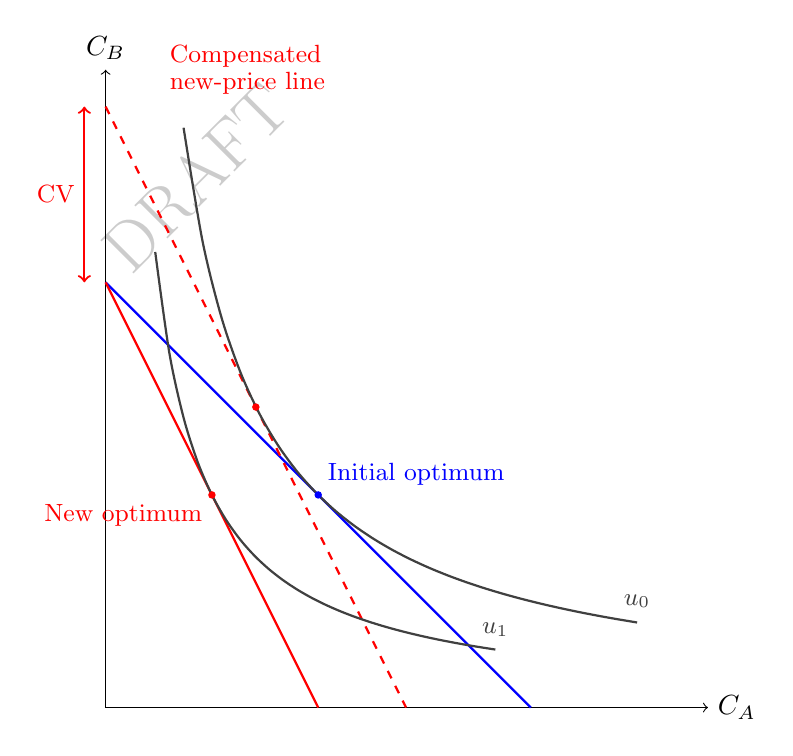
\begin{tikzpicture}[scale=0.9]
    % Axes
    \draw[->] (0,0) -- (8.5,0) node[right] {$C_A$};
    \draw[->] (0,0) -- (0,9.0) node[above] {$C_B$};

    % Budget lines
    \draw[thick, blue] (0,6) -- (6,0);


    \draw[thick, red] (0,6) -- (3,0);


    \draw[dashed, thick, red] (0,8.48) -- (4.24,0);
    \node[red, align=left] at (2.0,9.0) {\small Compensated\\[-0.5ex] \small new-price line};

    % Indifference curves
    \draw[domain=1.1:7.5,smooth,variable=\x, thick, darkgray] plot ({\x},{9/(\x)});
    \node[darkgray] at (7.5,1.5) {\small $u_0$};

    \draw[domain=0.7:5.5,smooth,variable=\x, thick, darkgray] plot ({\x},{4.5/(\x)});
    \node[darkgray] at (5.5,1.1) {\small $u_1$};

    % Tangency points
    \fill[blue] (3,3) circle (1.5pt) node[above right] {\small Initial optimum};
    \fill[red] (1.5,3) circle (1.5pt) node[below left] {\small New optimum};
    \fill[red] (2.12,4.24) circle (1.5pt);

    % CV arrow on vertical intercept
    \draw[<->, thick, red] (-0.3,6) -- (-0.3,8.48);
    \node[left, red] at (-0.3,7.24) {\small CV};
\end{tikzpicture}
\end{center}

\newpage
\paragraph{(ii) Equivalent variation.}
EV is the amount of income that could be taken away \emph{at the old prices} so that the consumer is just as badly off as after the price increase. Hence:
\begin{itemize}[leftmargin=*]
    \item the original budget line is tangent to \(u_0\);
    \item the new budget line is tangent to \(u_1\);
    \item an equivalent budget line, parallel to the original budget line, is shifted inward until it is tangent to \(u_1\).
\end{itemize}
The monetary gap between the original budget line and this inward-shifted old-price line is the equivalent variation.

\begin{center}
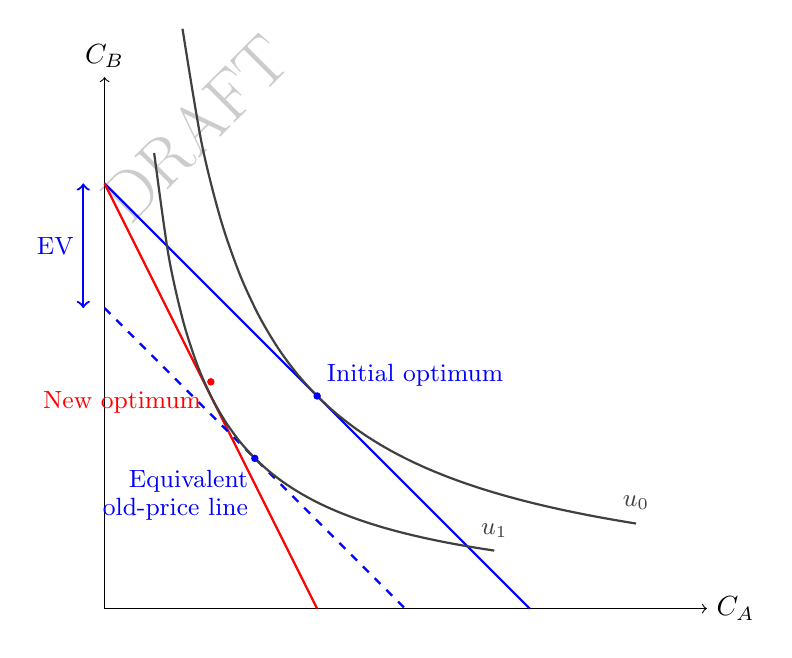
\begin{tikzpicture}[scale=0.9]
    % Axes
    \draw[->] (0,0) -- (8.5,0) node[right] {$C_A$};
    \draw[->] (0,0) -- (0,7.5) node[above] {$C_B$};

    % Budget lines
    \draw[thick, blue] (0,6) -- (6,0);


    \draw[thick, red] (0,6) -- (3,0);

    \draw[dashed, thick, blue] (0,4.24) -- (4.24,0);
    \node[blue, align=right] at (1,1.6) {\small Equivalent\\[-0.5ex] \small old-price line};

    % Indifference curves
    \draw[domain=1.1:7.5,smooth,variable=\x, thick, darkgray] plot ({\x},{9/(\x)});
    \node[darkgray] at (7.5,1.5) {\small $u_0$};

    \draw[domain=0.7:5.5,smooth,variable=\x, thick, darkgray] plot ({\x},{4.5/(\x)});
    \node[darkgray] at (5.5,1.1) {\small $u_1$};

    % Tangency points
    \fill[blue] (3,3) circle (1.5pt) node[above right] {\small Initial optimum};
    \fill[red] (1.5,3.2) circle (1.5pt) node[below left] {\small New optimum};
    \fill[blue] (2.12,2.12) circle (1.5pt);

    % EV arrow on vertical intercept
    \draw[<->, thick, blue] (-0.3,4.24) -- (-0.3,6);
    \node[left, blue] at (-0.3,5.12) {\small EV};
\end{tikzpicture}
\end{center}

These diagrams show the standard Hicksian welfare interpretation:
\[
\text{CV} = e(p_A',p_B,u_0)-e(p_A,p_B,u_0),
\qquad
\text{EV} = e(p_A,p_B,u_0)-e(p_A,p_B,u_1).
\]

\newpage
    \item
    For Cobb Douglas utility
    \[
    U(C_A,C_B)=C_A^{0.5}C_B^{0.5},
    \]
    the expenditure function is
    \[
    e(p_A,p_B,u)=2u\sqrt{p_Ap_B}.
    \]
    At the initial prices \((10,10)\) and income \(M=100\), the consumer spends half the income on each good, so
    \[
    C_A^*=\frac{50}{10}=5,
    \qquad
    C_B^*=\frac{50}{10}=5.
    \]
    Hence the initial utility is
    \[
    u_0=\sqrt{5\cdot 5}=5.
    \]

    CV is the extra income needed at the new prices \((20,10)\) to attain the original utility \(u_0=5\). Thus
    \[
    CV=e(20,10,5)-100.
    \]
    Compute:
    \[
    e(20,10,5)=2\cdot 5\sqrt{20\cdot 10}
    =10\sqrt{200}
    =10\cdot 10\sqrt{2}
    =100\sqrt{2}.
    \]
    Therefore
    \[
    CV=100\sqrt{2}-100=100(\sqrt{2}-1).
    \]
    Hence
    \[
    \boxed{CV=100(\sqrt{2}-1).}
    \]

    \item
    No, EV will not be equal to CV in this case.

    The reason is that Cobb Douglas preferences are \emph{not} quasilinear, so demand exhibits income effects. Fruit A is a normal good under Cobb Douglas preferences, and the price increase is harmful. For a price increase of a normal good, restoring the consumer to the original utility at the new prices is more expensive than measuring the equivalent utility loss at the old prices. Hence
    \[
    CV>EV.
    \]

    Therefore
    \[
    \boxed{EV\neq CV,\qquad CV>EV.}
    \]
\end{enumerate}

\newpage
\subsubsection{Method 2: Hicksian minimisation method}
\begin{enumerate}[label=(\alph*)]
    \item
    The graphical interpretation is the same as in Method 1.

    For CV, use the \emph{new} price slope and restore the \emph{old} indifference curve.  
    For EV, use the \emph{old} price slope and reduce income until the \emph{new} indifference curve is just reached.

    More precisely:
    \[
    \text{CV uses }(p_A',p_B)\text{ and }u_0,
    \qquad
    \text{EV uses }(p_A,p_B)\text{ and }u_1.
    \]

    \item
    At the initial prices \((10,10)\) and income \(100\), Cobb Douglas expenditure shares imply
    \[
    C_A^*=5,\qquad C_B^*=5,
    \]
    so
    \[
    u_0=\sqrt{5\cdot 5}=5.
    \]

    To compute CV, solve the Hicksian problem at the new prices:
    \[
    \min_{C_A,C_B>0}\;20C_A+10C_B
    \qquad\text{subject to}\qquad
    C_A^{0.5}C_B^{0.5}=5.
    \]
    Equivalently,
    \[
    C_AC_B=25.
    \]
    Substitute
    \[
    C_B=\frac{25}{C_A}
    \]
    into expenditure:
    \[
    E(C_A)=20C_A+10\left(\frac{25}{C_A}\right)
    =20C_A+\frac{250}{C_A}.
    \]
    Differentiate:
    \[
    E'(C_A)=20-\frac{250}{C_A^2}.
    \]
    Setting \(E'(C_A)=0\),
    \[
    20=\frac{250}{C_A^2}
    \quad\Longrightarrow\quad
    C_A^2=\frac{25}{2}
    \quad\Longrightarrow\quad
    C_A=\frac{5}{\sqrt2}.
    \]
    Then
    \[
    C_B=\frac{25}{5/\sqrt2}=5\sqrt2.
    \]
    Thus minimum expenditure is
    \[
    20\left(\frac{5}{\sqrt2}\right)+10(5\sqrt2)
    =50\sqrt2+50\sqrt2
    =100\sqrt2.
    \]
    Hence
    \[
    CV=100\sqrt2-100=100(\sqrt2-1).
    \]
    Therefore
    \[
    \boxed{CV=100(\sqrt2-1).}
    \]

    \item
    At the new prices \((20,10)\) and income \(100\), the Marshallian bundle is
    \[
    C_A'=\frac{50}{20}=2.5,
    \qquad
    C_B'=\frac{50}{10}=5.
    \]
    Hence the new utility is
    \[
    u_1=\sqrt{2.5\cdot 5}=\frac{5}{\sqrt2}.
    \]

    Since preferences are Cobb Douglas, there are income effects. Therefore EV and CV are not equal in general. Moreover, because fruit A is a normal good and its price rises,
    \[
    CV>EV.
    \]
    Hence
    \[
    \boxed{EV\neq CV,\qquad CV>EV.}
    \]
\end{enumerate}


%====================================================
% QUESTION 6 / Sample Question 2
%====================================================
\newpage
\section{Sample Question 2: Bob, Quasi-linear Utility, and Reservation Prices}

\noindent
Bob, who has wealth of \(w\) is deciding where to go for tea-time. There are \(3\) possible options, i) \(X\), ii) \(Y\), iii) \(Z\), and he can choose only \(1\) of the options.

\medskip

\noindent
If he chooses an option, its value is \(1\). If he does not choose the option, its value is \(0\). For example, if he chooses \(Y\), then \(X=0\), \(Y=1\), \(Z=0\) and so on.

\medskip

\noindent
His utility depends on which item he chooses and his leftover holdings of cash \(m\) as follows:
\[
u(X,Y,Z,m)=a\sqrt{X}+b\sqrt{Y}+c\sqrt{Z}+dm,
\]
where \(a,b,c,d>0\).

\subsection{Problem}
\begin{enumerate}[label=(\alph*)]
    \item State the definition of quasi-linear utility. Is Bob’s utility quasi-linear?
    \item Solve for Bob’s reservation prices for option \(X\), option \(Y\) and option \(Z\).
\end{enumerate}

\bigskip
\subsection{Solution}

\subsubsection{Method 1: Definition and indifference-pricing method}
\begin{enumerate}[label=(\alph*)]
    \item
    A utility function is \emph{quasi-linear} if it can be written in the form
    \[
    u(q,m)=\phi(q)+m
    \]
    up to a positive affine rescaling of the money variable, where utility is linear in one good, usually money.

    Here,
    \[
    u(X,Y,Z,m)=a\sqrt{X}+b\sqrt{Y}+c\sqrt{Z}+dm.
    \]
    Since \(d>0\), this is linear in money \(m\). Therefore Bob’s utility is quasi-linear. Equivalently, one may write
    \[
    u(X,Y,Z,m)=\phi(X,Y,Z)+dm,
    \]
    where
    \[
    \phi(X,Y,Z)=a\sqrt{X}+b\sqrt{Y}+c\sqrt{Z}.
    \]
    Hence
    \[
    \boxed{\text{Bob’s utility is quasi-linear.}}
    \]

\newpage
    \item
    Since \(X,Y,Z\in\{0,1\}\), we have
    \[
    \sqrt{X}=X,\qquad \sqrt{Y}=Y,\qquad \sqrt{Z}=Z.
    \]
    So the utility may be simplified to
    \[
    u(X,Y,Z,m)=aX+bY+cZ+dm.
    \]

    The reservation price for option \(X\) is the maximum amount Bob is willing to pay to choose \(X\) rather than choose no option. If he chooses no option, his utility is
    \[
    u(0,0,0,w)=dw.
    \]
    If he chooses option \(X\) and pays price \(r_X\), then his leftover cash is \(w-r_X\), so his utility is
    \[
    u(1,0,0,w-r_X)=a+d(w-r_X).
    \]
    At the reservation price he is indifferent:
    \[
    a+d(w-r_X)=dw.
    \]
    Hence
    \[
    dr_X=a
    \quad\Longrightarrow\quad
    \boxed{r_X=\frac{a}{d}.}
    \]

    Similarly, for option \(Y\),
    \[
    u(0,1,0,w-r_Y)=b+d(w-r_Y),
    \]
    and indifference with choosing no option gives
    \[
    b+d(w-r_Y)=dw
    \quad\Longrightarrow\quad
    \boxed{r_Y=\frac{b}{d}.}
    \]

    Likewise, for option \(Z\),
    \[
    u(0,0,1,w-r_Z)=c+d(w-r_Z),
    \]
    so
    \[
    c+d(w-r_Z)=dw
    \quad\Longrightarrow\quad
    \boxed{r_Z=\frac{c}{d}.}
    \]

    Therefore
    \[
    \boxed{
    r_X=\frac{a}{d},\qquad
    r_Y=\frac{b}{d},\qquad
    r_Z=\frac{c}{d}.
    }
    \]
\end{enumerate}

\newpage
\subsubsection{Method 2: Utility-value conversion method}
\begin{enumerate}[label=(\alph*)]
    \item
    A utility function is quasi-linear if utility is linear in one argument, typically money. Here
    \[
    u(X,Y,Z,m)=a\sqrt{X}+b\sqrt{Y}+c\sqrt{Z}+dm
    \]
    is linear in \(m\), so Bob’s utility is quasi-linear.

    Hence
    \[
    \boxed{\text{Bob’s utility is quasi-linear.}}
    \]

    \item
    Since one extra dollar of leftover cash raises utility by
    \[
    d,
    \]
    the marginal utility of money is \(d\). Therefore a utility increment of size \(\Delta u\) has money equivalent
    \[
    \frac{\Delta u}{d}.
    \]

    Now the utility bonus from choosing option \(X\) rather than no option is
    \[
    a\sqrt{1}=a.
    \]
    So its reservation price is
    \[
    \boxed{r_X=\frac{a}{d}.}
    \]

    Similarly, option \(Y\) gives utility bonus
    \[
    b\sqrt{1}=b,
    \]
    so
    \[
    \boxed{r_Y=\frac{b}{d}.}
    \]

    Option \(Z\) gives utility bonus
    \[
    c\sqrt{1}=c,
    \]
    so
    \[
    \boxed{r_Z=\frac{c}{d}.}
    \]

    Therefore
    \[
    \boxed{
    r_X=\frac{a}{d},\qquad
    r_Y=\frac{b}{d},\qquad
    r_Z=\frac{c}{d}.
    }
    \]
\end{enumerate}

\newpage
\subsubsection{Method 3: Binary-choice simplification method}
\begin{enumerate}[label=(\alph*)]
    \item
    Because each of \(X,Y,Z\) is binary,
    \[
    X,Y,Z\in\{0,1\},
    \]
    the square-root terms simplify exactly:
    \[
    \sqrt{X}=X,\qquad \sqrt{Y}=Y,\qquad \sqrt{Z}=Z.
    \]
    Hence Bob’s utility can be rewritten as
    \[
    u(X,Y,Z,m)=aX+bY+cZ+dm.
    \]
    This is of quasi-linear form: an additive term depending on the discrete choice variables plus a linear money term.

    Therefore
    \[
    \boxed{\text{Bob’s utility is quasi-linear.}}
    \]

    \item
    In the simplified form
    \[
    u(X,Y,Z,m)=aX+bY+cZ+dm,
    \]
    choosing no option yields utility
    \[
    dw.
    \]
    Choosing option \(X\) and paying price \(p\) yields
    \[
    a+d(w-p).
    \]
    Bob is indifferent when
    \[
    a+d(w-p)=dw
    \quad\Longrightarrow\quad
    p=\frac{a}{d}.
    \]
    So
    \[
    \boxed{r_X=\frac{a}{d}.}
    \]

    Repeating the same argument for \(Y\) and \(Z\),
    \[
    \boxed{r_Y=\frac{b}{d},\qquad r_Z=\frac{c}{d}.}
    \]

    Therefore
    \[
    \boxed{
    r_X=\frac{a}{d},\qquad
    r_Y=\frac{b}{d},\qquad
    r_Z=\frac{c}{d}.
    }
    \]
\end{enumerate}
\end{document}